\chapter{Het integreren van logica in de ontwerptaal voor sequentiediagrammen}\label{sec:decl-seq}
UML is een modelleertaal die wordt gebruikt ter ondersteuning van softwareontwerp in imperatieve programmeertalen. In sequentiediagrammen vertaalt zich dat tot een veelvoud aan instructies voor eenvoudige taken zoals het selecteren van het eerste getal verschillend van 0 in een lijst van getallen. Aangezien elke nieuwe instructie in een sequentiediagram leidt tot minstens \'e\'en zin in de gegenereerde theorie, impliceert dit een grote kost in zowel rekentijd als geheugengebruik voor modelexpansie en progressie\"inferentie, zoals we hebben aangetoond in hoofdstuk \ref{sec:evaluatie}. Daarom geven we in dit hoofdstuk een aanzet tot het integreren van logica in het ontwerp van sequentiediagrammen.

\section{Vergelijking tussen lineaire tijdcalculus en onze voorstellingsmethode}

We modelleren eerst Nim rechtstreeks in lineaire tijdcalculus en vergelijken de resulterende theorie met de theorie gegenereerd volgens de regels in hoofdstuk \ref{sec:gedrag}. Het volgende codefragment bevat een LTC-theorie die Nim modelleert. 

\lstinputlisting[caption=Nim gemodelleerd in lineaire tijdcalculus]{chap-declaratieve-seq/ltc-nim.idp}\label{code:ltc-nim}

Bij het opstellen van deze theorie werden de volgende stappen gevolgd:

\begin{enumerate}
	\item Bepaal de variabelen die de toestand van het systeem beschrijven. Zo krijgen we de logische types \textit{Heap}, die stapels voorstellen; \textit{Size}, wat het aantal objecten op een stapel voorstelt; en \textit{Player}, voorgesteld door exact twee getallen voor de twee spelers. We onderscheiden ook de functies \textit{NumObj(Time, Heap) : Size}, wat de grootte van een stapel op een bepaald tijdstip voorstelt; en \textit{PlayerTurn(Time) : Player}, die voor elk tijdstip aangeeft welke speler aan beurt is. Deze functies maken we inertieel.
	\item Bepaal welke bewerkingen er kunnen gebeuren op het systeem op elk tijdstip die er mogelijks voor zorgen dat de toestand van het systeem verandert in toekomstige tijdstappen. Definieer de \textit{constructed type Action} die deze bewerkingen benoemt. Voor Nim is er maar \'e\'en actie mogelijk: het nemen van een aantal objecten van een bepaalde stapel. Daarom defini\"eren we het type \textit{Action} met behulp van de Herbrandfunctor \textit{Take(Heap, Size)}. Dit garandeert het uniekenaamaxioma en domeinsluitingsaxioma voor het type \textit{Action} in termen van logische objecten van het type \textit{Heap} en het type \textit{Size}.\cite{DeCatBroes2014PLaa} Met andere woorden: elk mogelijk tupel $(h, s)$ waar $h \in Heap$ en $s \in Size$ correspondeert met \'e\'en uniek logisch object $Take(h, s)$. Het domein van het type \textit{Action} bestaat uitsluitend uit deze objecten.
	\item Leg geschikte voorwaarden op de uitvoering van de bewerkingen bepaald in de vorige stap. In Nim moeten we ervoor zorgen dat een speler objecten neemt van een niet-lege stapel en dat een speler minstens \'e\'en object wegneemt van de gekozen stapel. De speler mag niet meer objecten wegnemen dan aanwezig op de stapel.
	\item Schrijf de causatiezinnen. Specificeer hoe een bewerking de toestand van het systeem verandert. We leiden af dat \textit{NumObj} verandert ten gevolge van een \textit{Take} actie. Verder zorgen we ervoor dat er elke tijdstap een beurtwissel gebeurt.
	\item Schrijf de toestandzinnen. Deze hebben een vast patroon voor elk inertieel logisch symbool.
\end{enumerate}

Het meest opmerkelijk verschil tussen deze logische specificatie en de specificatie in bijlage \ref{code:nim-eval} is dat zowel het vocabularium en de theorie significant compacter zijn. De combinatie van kleinere zoekruimte en minder zinnen om rekening mee te houden zorgt ervoor dat zowel rekentijd als geheugengebruik sterk verkleinen. Inderdaad, voor een spel met een stapel met twee objecten en een stapel met drie objecten duurt het iets meer dan twee seconden om alle 37 mogelijke spelverlopen te vinden. Daarbij is de \textit{grounding}-grootte 3855 en het virtueel geheugengebruik 40,59 MB. Vergelijk met de verificatie van \textit{allHeapsEmpty} in hoofdstuk \ref{sec:evaluatie}, waar de rekentijd 43,29 seconden was, de \textit{grounding}-grootte 366 643 en het virtueel geheugengebruik 1,63 GB.

We merken op dat een belangrijk nadeel dat sequentiediagrammen hebben ten opzichte van rechtstreekse LTC is dat de toestand van maar \'e\'en variabele kan opgevraagd of aangepast worden. De LTC-theorie heeft bijvoorbeeld \'e\'en zin nodig om te verzekeren dat het spel voorbij is indien alle stapels leeg zijn. Er is echter een heel diagram nodig om voor elke stapel om de beurt te controleren of die leeg is.

Verder kan de LTC-theorie ook meteen alle lege stapels uitsluiten wanneer de speler moet kiezen van welke stapel hij objecten neemt. In figuur \ref{fig:nim-takeTurn} moet eerst gecontroleerd worden of de stapel die de speler kiest effectief leeg is. Het keuzeproces herhaalt zich tot de gebruiker een niet-lege stapel kiest. Zulk een iteratief proces is niet aanwezig in de LTC-theorie. Beschouw ook het diagram \ref{fig:nim-allHeapsEmpty} dat \textit{allHeapsEmpty()} modelleert. Daar controleert de lus voor elke stapel om de beurt of hij leeg is. Deze iteratieve controle is niet aanwezig in de LTC-theorie.

We stellen de volgende zaken vast:

\begin{enumerate}
	\item Indien een LTC-theorie een iteratief proces bevat, komt dit overeen met een iteratief proces in het beschouwde probleemdomein. In listing \ref{code:ltc-nim} is de beurtenwissel het enige iteratief proces. Dit is ook het enige iteratief proces dat bestaat in Nim.
	\item De modellering van Nim in sectie \ref{sec:nim-design} bevat naast de beurtenwissel ook iteratieve processen die niet overeenkomen met een proces in Nim. Zulke processen zijn ook aanwezig in het ontwerp voor Reversi in sectie \ref{sec:reversi-design}. Een voorbeeld daarvan is het diagram voor \textit{count(Player)}, dat elk speelvak afgaat om te tellen hoeveel stenen een bepaalde speler op het bord heeft liggen. Dit komt niet overeen met een iteratief proces in Reversi. Modelleringen volgens onze voorstelling zullen dus zowel iteratieve processen die overeenkomen met een proces in het probleemdomein bevatten als iteratieve processen die een berekening uitvoeren die niet rechtstreeks relevant is voor het probleemdomein.
\end{enumerate}

De extra iteratieve processen in onze voorstelling leiden tot nieuwe logische symbolen die de variabelen betrokken in het proces voorstellen. De theorie zal ook zinnen bevatten die overeenkomen met bewerkingen op die variabelen. Zulke processen vergroten op deze manier de rekentijd en het geheugengebruik voor modelexpansie en progressie\"inferentie.

Deze observaties leiden ertoe dat we nieuwe soorten instructies voor sequentiediagrammen beschikbaar willen stellen met het oog op deze doelen:

\begin{enumerate}
	\item Het totale aantal instructies over alle sequentiediagrammen verminderen
	\item Het aantal LTC-tijdstappen die nodig zijn bij modelexpansie of progressie\"inferentie om een bepaalde taak te verrichten verminderen
\end{enumerate}

Concreet willen we instructies die ons toelaten om de toestand van alle objecten in een verzameling op te vragen, te controleren of te wijzigen. Verder willen we ook instructies die bij simulatie toelaten om te kiezen uit bepaalde leden uit een verzameling op basis van een criterium op de toestand van de leden.

\section{Nieuwe soorten instructies}\label{sec:new-instr}

Voorheen kon een variabele maar \'e\'en object of waarde van een primitief type voorstellen. Nu laten we toe dat een variabele een verzameling kan voorstellen. In de theorie behouden we voor namen het patroon $<variabelenaam>T/3$.

\subsubsection{Nieuwe toegelaten instructies in sequentiediagrammen}

We laten de volgende nieuwe instructies toe in sequentiediagrammen:

\begin{enumerate}
	\item Voor alle leden van een verzameling tegelijkertijd kan een associatie genavigeerd worden. Als op een verzameling S van objecten van klasse X \textit{getY()} wordt uitgevoerd waar Y de naam is van een klasse geassocieerd met X, dan is het resultaat een verzameling van objecten van klasse Y. Die verzameling bestaat uit alle objecten die in verband staan met minstens \'e\'en object uit S.
	\item $getNumX()$ waar X de naam is van een klasse die in verband staat met de klasse van de verzameling. Het resultaat is de som van het aantal instanties van klasse X waarmee elk lid van de verzameling in verband staat.
	\item $EXISTS\ ONE\ [x]\ FROM\ [y]\ WHERE\ [query]$: $y$ stelt een verzameling voor. $x$ wordt gebonden in $query$ en stelt een lid van $y$ voor. \textit{query} stelt een instructie voor die bestaat uit getters van klassevariabelen verbonden met booleaanse connectieven. Klassevariabelen kunnen hierbij rechtstreeks vergeleken worden met een getal of string, waar toepasselijk. Deze instructie geeft \textbf{true} als en slechts als minstens \'e\'en $x$ bestaat waarvoor \textit{query} geldt.\label{instr:exists-one}
	\item $EXISTS\ n\ TO\ m\ [x]\ FROM\ [y]\  WHERE\ [query]$ waar $n \leq m$: Geeft \textbf{true} als en slechts als \textit{query} geldt voor minstens $n$ en ten hoogste $m$ verschillende waarden $x \in y$. Het domein voor $n$ en $m$ is $[1,+\infty]$.
	\item $FOR\ ALL\ [x]\ FROM\ [y]\ APPLIES\ [query]$: Geeft \textbf{true} als en slechts als $query$ geldt voor alle $x \in y$.
	\item $NOT\ [query]$: geeft \textbf{true} als en slechts als \textit{query} \textbf{false} geeft. \textit{query} kan hier \'e\'en van de voorgaande soorten instructies zijn.
	\item $CHOOSE\ ALL\ [x]\ FROM\ [y]\ WHERE\ APPLIES\ [query]$: Geeft een nieuwe verzameling die bestaat uit alle $x \in y$ waarvoor \textit{query} waar is.
	\item $CHOOSE\ ONE\ [x]\ FROM\ [y]\ WHERE\ APPLIES\ [query]$: Geeft \'e\'en $x \in y$ waarvoor \textit{query} waar is. Dit vormt een keuzepunt bij simulatie.\label{instr:choose-one}
	\item $CHOOSE\ n\ TO\ m\ [x]\ FROM\ [y]\ WHERE\ APPLIES\ [query]$ waar $1 \leq n \leq m < +\infty$: Geeft een nieuwe verzameling die bestaat uit minstens $n$ en ten hoogste $m$ $x \in y$ waarvoor \textit{query} waar is. Dit vormt een keuzepunt bij simulatie.\label{instr:choose-n-to-m}
	\item $SET <klassevariabele> IN\ [y]\ TO <waarde>$: Voor alle leden van de verzameling wordt de waarde van de genoemde klassevariabele veranderd naar de genoemde waarde.\label{instr:set}
\end{enumerate}

In instructies \ref{instr:exists-one} tot en met \ref{instr:set} kan $y$ een verzameling van alle waarden van een primitief type zijn, zoals ``Integer'', ``Float'' of ``String''.

In een \textit{query} mogen er geen methodes voorkomen waarvan het gedrag gespecificeerd wordt in een sequentiediagram.

\subsubsection{Vergelijking van de \textit{CHOOSE}-instructies met de $\pi$-operator in GOLOG}

GOLOG\cite{levesque1997golog} is een logische programmeertaal gebaseerd op de situatiecalculus. Net zoals de lineaire tijdscalculus is de situatiecalculus een formalisme binnen de eerste-orde-predicatenlogica om dynamische systemen te modelleren. De basisblokken van de situatiecalculus zijn:

\begin{itemize}
	\item De acties die uitgevoerd kunnen worden in het systeem.
	\item De \textit{fluents} die de toestand van het systeem beschrijven.
	\item De situaties. Een situatie is een geschiedenis van uitgevoerde acties.
\end{itemize}

De $\pi$-operator is de non-deterministische keuzeoperator, gebruikt als $(\pi{}x)[\delta{}(x)]$, waar $\delta{}(x)$ \'e\'en of meerdere acties die de variabele $x$ binden voorstelt. De $\pi$-operator bepaalt non-deterministisch de waarde van het invoerargument voor de acties waar het op wordt toegepast. Als \textit{pickup(x)} bijvoorbeeld een actie voorstelt waarbij een robot een object opraapt, kiest $(\pi{}x)[pickup(x)]$ op non-deterministische wijze het object $x$ dat de robot opraapt. Instructies \ref{instr:choose-one} en \ref{instr:choose-n-to-m} zijn gelijkaardig. De gebruiker kiest uit alle $x \in y$ die voldoen aan een voorwaarde die $x$ bindt. De keuze van de gebruiker wordt dan toegekend aan een variabele. 

\subsubsection{Modellering van Nim met de nieuwe instructies}

We illustreren het gebruik van deze nieuwe instructies door middel van het voorbeeld van figuur \ref{fig:new-nim}, dat Nim volledig modelleert. De beurt gaat eerst naar de gekozen speler. Dan wordt gecontroleerd of alle stapels leeg zijn. Als dat niet het geval is, kiest de speler eerst een stapel en neemt dan minstens \'e\'en object weg van die stapel. Daarna wordt de beurt gegeven aan de volgende speler. Als alle stapels leeg zijn, is de huidige speler de winnaar.

\begin{figure}[H]
	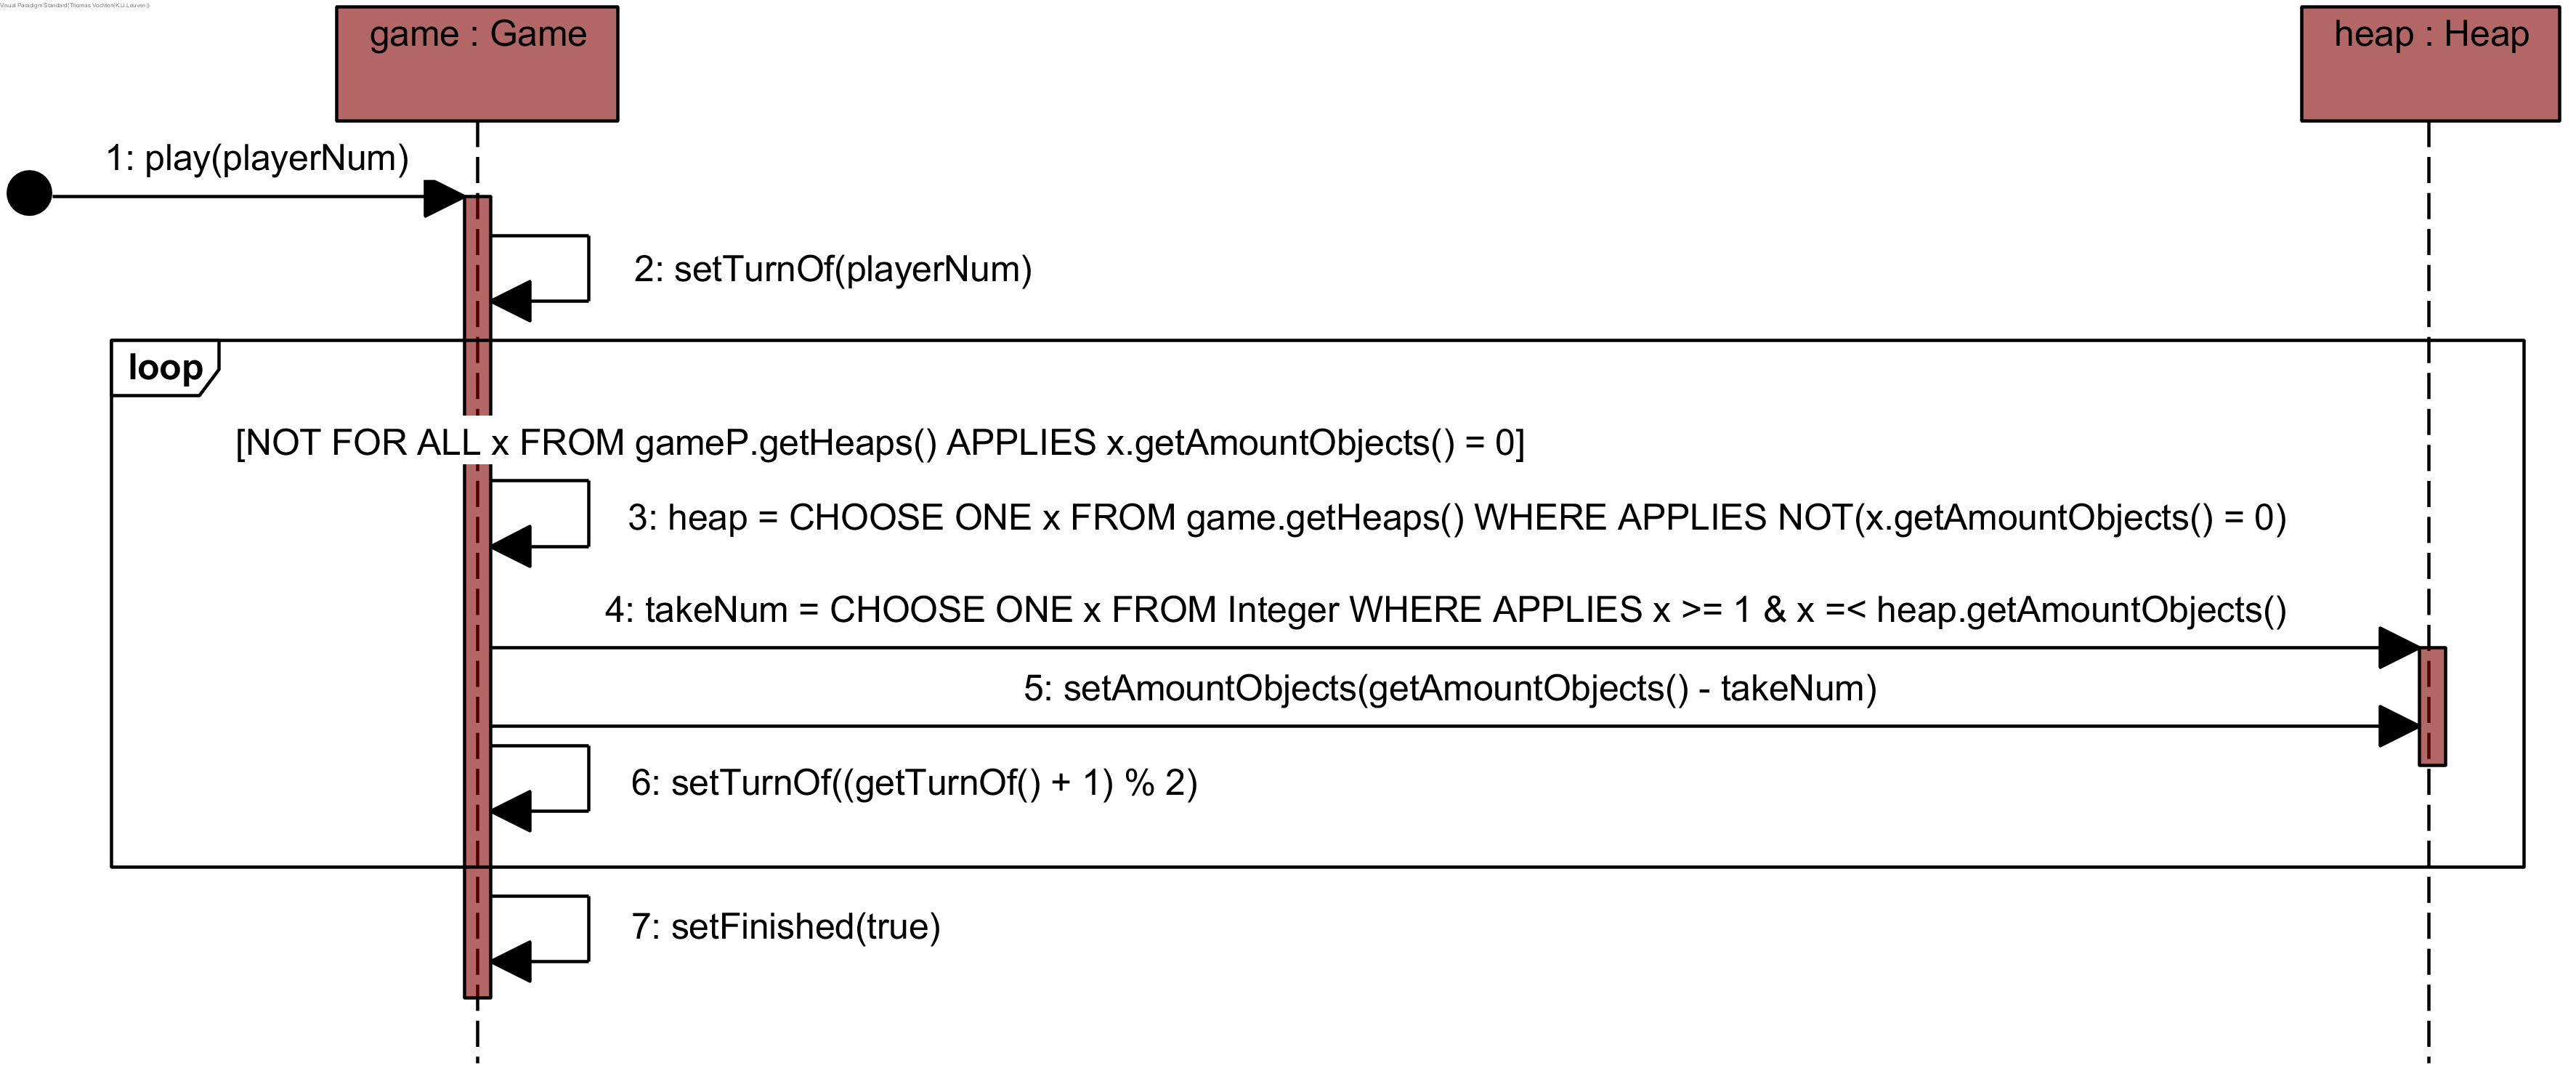
\includegraphics[width=\textwidth]{chap-gedrag/seq-new-nim.png}
	\caption{Een modellering van het spel Nim}
	\label{fig:new-nim}
\end{figure}

De lusvoorwaarde wordt als volgt voorgesteld:

\begin{align}
\nonumber &\forall{t}[Time]\forall{st}[StackLevel](C\_SDPointAt(Next(t), play\_3) \leftarrow \\ \nonumber &(CurrentStackLevel(t) = st) \land (SDPointAt(t, play\_2) \lor SDPointAt(t, play\_6)) \land \\ \nonumber &\lnot{}\exists{g}[Game](GameT(t, st, g) \land{}\forall{h}[Heap](GameandHeap(g, h) \\ &\Rightarrow \exists{n}[LimitedInt](HeapamountObjects(t, h, n) \land n = 0)))). \\
\nonumber &\forall{t}[Time]\forall{st}[StackLevel](C\_SDPointAt(Next(t), play\_7) \leftarrow \\ \nonumber &(CurrentStackLevel(t) = st) \land SDPointAt(t, play\_6) \land \exists{g}[Game](GameT(t, st, g) \land \\ \nonumber &\forall{h}[Heap](GameandHeap(g, h) \\ &\Rightarrow \exists{n}[LimitedInt](HeapamountObjects(t, h, n) \land n = 0)))).
\end{align}

In instructie 3 wordt de $CHOOSE\ ONE\ WHERE\ APPLIES\ [query]$ instructie gebruikt. We introduceren hier een open predicaat, $ChosenHeap(Time, Heap)$, om ons te helpen deze instructie te vertalen. We voegen de volgende zin toe aan het definitieblok voor diagramvariabelen:

\begin{align}
\nonumber &\forall{t}[Time]\forall{st}[StackLevel]\forall{h}[Heap](C\_HeapT(Next(t), st, h) \\ &\leftarrow (CurrentStackLevel(t) = st) \land SDPointAt(t, play\_3) \land ChosenHeap(t, h)).
\end{align}

Om ervoor te zorgen dat exact \'e\'en Heap-object wordt gekozen, moeten we voorwaardes leggen op $ChosenHeap/2$. Dit doen we als volgt:

\begin{align}
&\forall{t}[Time](SDPointAt(t, play\_3) \Rightarrow \exists_{=1}{h}[Heap](ChosenHeap(t, h))).\label{form:uniqueheap} \\
\nonumber &\forall{t}[Time]\forall{h}[Heap](ChosenHeap(t, h) \Rightarrow (SDPointAt(t, play\_3) \\ \nonumber &\land \exists{g}[Game]\exists{st}[StackLevel]\exists{n}[LimitedInt]((CurrentStackLevel(t) = st) \\ &\land GameT(t, st, g) \land GameandHeap(g, h) \land HeapamountObjects(t, h, n) \land \lnot(n = 0)))).\label{form:correctsd}
\end{align}

Zin \ref{form:uniqueheap} garandeert dat er maar \'e\'en \textit{Heap}-object mag gekozen worden.

Zin \ref{form:correctsd} garandeert dat er enkel een keuze mag gemaakt worden als de uitvoering instructie 3 bereikt en dat er enkel een \textit{Heap}-object wordt gekozen waarvoor geldt dat \textit{amountObjects} groter is dan 0.

Voor instructie 4 introduceren we op een soortgelijke manier een open predicaat $ChosenTake/2$. De zin die we toevoegen aan het definitieblok voor variabelen en de voorwaarden die we opleggen op $ChosenTake/2$ zien er gelijkaardig uit.

Bijlage \ref{code:new-nim} bevat de vertaling van het diagram in figuur \ref{fig:new-nim}.

\section{Performantie van modelexpansie en progressie\"inferentie}\label{sec:dec-performance}

We beoordelen voor de theorie in bijlage \ref{code:new-nim} de rekentijd en het geheugengebruik voor modelexpansie en progressie\"inferentie.

Voor modelexpansie specificeren we in de invoerstructuur \'e\'en stapel met twee objecten en \'e\'en stapel met drie objecten. Het scenario is dus analoog aan die in hoofdstuk \ref{sec:evaluatie}. Verder defini\"eren we 11 tijdstappen, wat genoeg is voor twee beurten. Het duurt ongeveer 5,8 seconden om een volledig spelverloop te berekenen, met een \textit{grounding}-grootte van 15 249 en virtueel geheugengebruik van 71,18 MB. Modelexpansie is dus significant performanter voor deze theorie dan voor de theorie ge\"evalueerd in hoofdstuk \ref{sec:evaluatie}.

We simuleren weer een spelverloop waar de eerste speler alle drie objecten van de tweede stapel neemt, dan de tweede speler \'e\'en object van de eerste stapel, en dan de eerste speler het laatste object. In totaal is de simulatie 16 tijdstappen lang, met een totale simulatietijd van 93,11 seconden en een totaal geheugengebruik van 242,3 MB. Als we dit vergelijken met de resultaten in tabel \ref{tab:sim-mem}, zien we dat zowel de simulatietijd als het geheugengebruik significant kleiner zijn.

\section{Variabele associaties}\label{sec:var-assoc}

Sectie \ref{sec:eval-design} besprak hoe het feit dat de invulling van een associatie niet kan veranderen over de tijd tot onintu\"itieve ontwerpen leidt. We legden die beperking op om de rekentijd en het geheugengebruik bij modelexpansie en progressie\"inferentie beperkt te houden. Na de resultaten in sectie \ref{sec:dec-performance} onderzoeken we wat het effect is op de rekentijd en het geheugengebruik als we deze beperking opheffen nu de instructies uit sectie \ref{sec:new-instr} beschikbaar zijn.

Associaties defini\"eren nu impliciet twee operaties. Voor een associatie \textit{X}---\textit{Y} wordt voor de klasse \textit{X} de operatie \textit{setY(Y)} en de operatie \textit{unset(Y)} gedefinieerd. \textit{setY(Y)} relateert het object van klasse \textit{X} tot het gegeven object van klasse \textit{Y}. \textit{unsetY(Y)} zorgt ervoor dat het object niet meer gerelateerd is aan het gegeven object.

We maken weer een nieuw ontwerp voor Nim.

Figuur \ref{fig:nim-assoc-cd} toont het klassediagram. Er is een nieuwe klasse vergeleken met het ontwerp in sectie \ref{sec:nim-design}, namelijk \textit{Player}. De associatie \textit{Game}---\textit{Player} duidt de winnaar aan.

Figuur \ref{fig:nim-assoc-play} geeft het sequentiediagram voor \textit{play(Player, Player)}. De lus wordt uitgevoerd zolang nog niet alle stapels leeg zijn. Eerst krijgt \textit{player1} de beurt en daarna \textit{player2} als er nog een niet-lege stapel is. Instructie 3 markeert \textit{player2} als de winnaar indien \textit{player1} het laatste object neemt. Instructie 5 doet hetzelfde voor \textit{player1}.

Figuur \ref{fig:nim-assoc-taketurn} toont het sequentiediagram voor \textit{takeTurn(Game)}. De speler kiest een niet-lege stapel en neemt minstens \'e\'en object ervan weg.

Bijlage \ref{app:nim-assoc} bevat het IDP-bestand dat deze diagrammen modelleert. De predicaten die de associaties voorstellen, namelijk \textit{GameandHeap} en \textit{GameandPlayer}, zijn inertieel. Zo laten we toe dat associaties variabel zijn over de tijd.

\begin{figure}
	\centering
	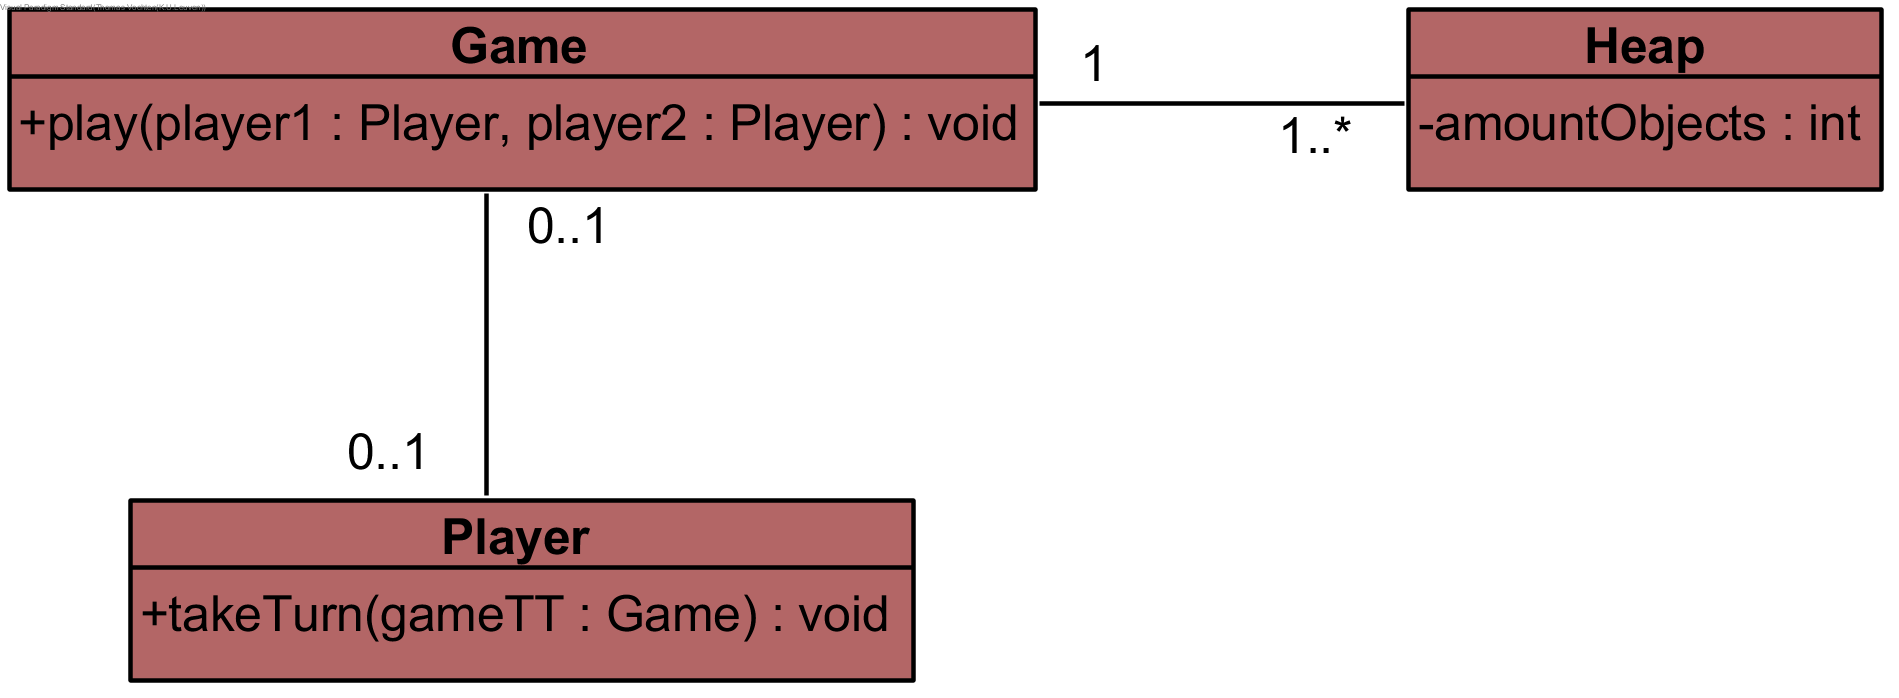
\includegraphics[width=0.75\textwidth]{chap-declaratieve-seq/nim-assoc-cd.png}
	\caption{Klassediagram voor Nim, met een extra klasse \textit{Player}}
	\label{fig:nim-assoc-cd}
\end{figure}

\begin{figure}
	\centering
	\begin{subfigure}{\textwidth}
		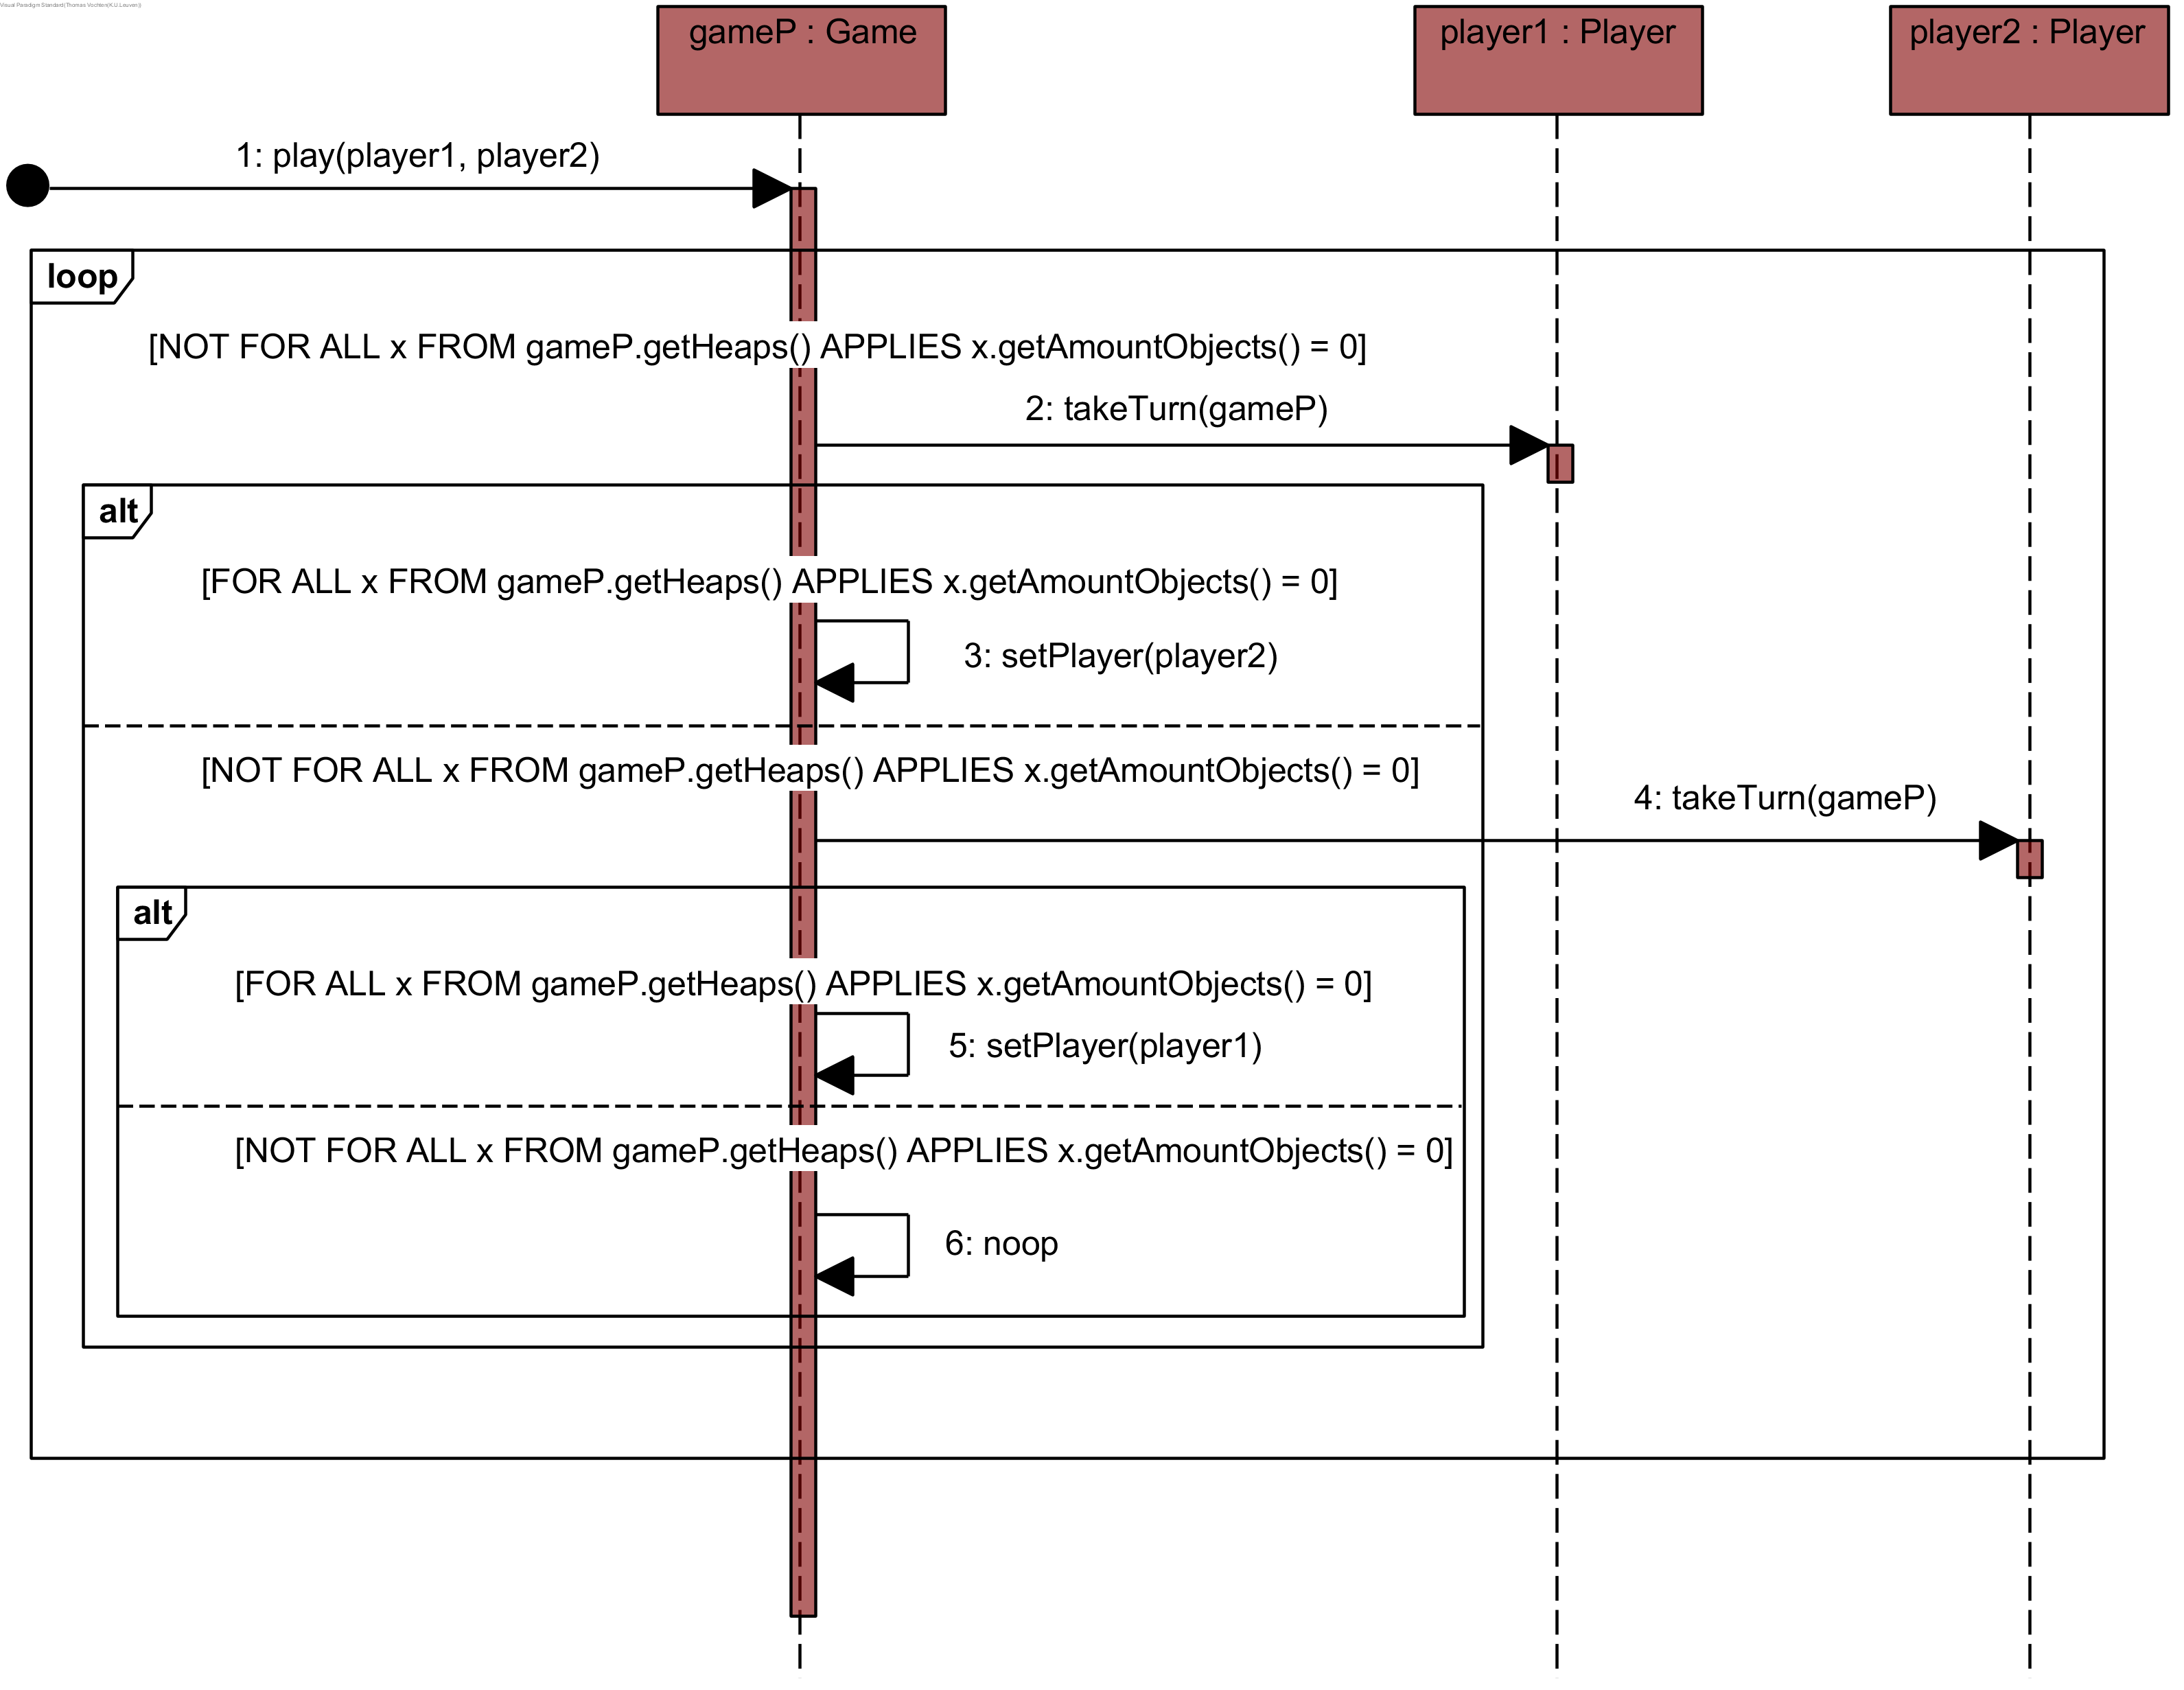
\includegraphics[width=\textwidth]{chap-declaratieve-seq/play.png}
		\caption{Sequentiediagram voor \textit{play(Player, Player)}}
		\label{fig:nim-assoc-play}
	\end{subfigure}
	\begin{subfigure}{\textwidth}
		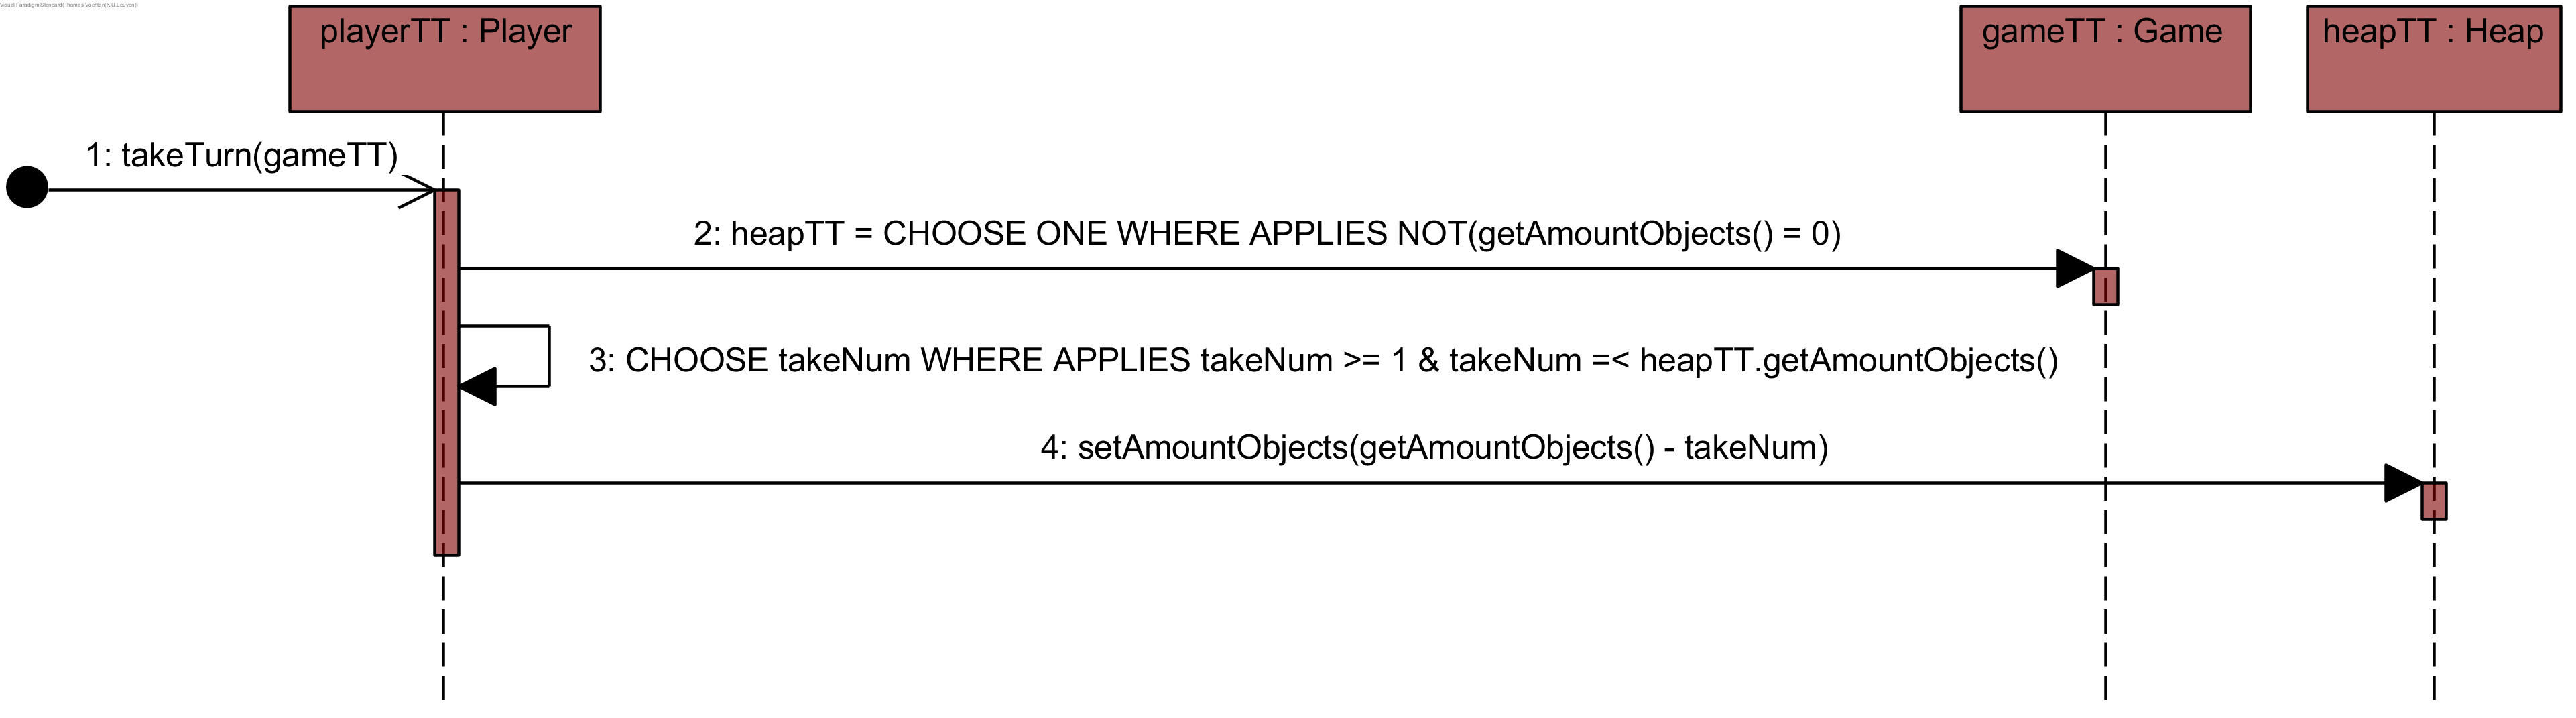
\includegraphics[width=1.1\textwidth]{chap-declaratieve-seq/takeTurn.png}
		\caption{Sequentiediagram voor \textit{takeTurn(Game)}}
		\label{fig:nim-assoc-taketurn}
	\end{subfigure}
	\caption{Sequentiediagrammen voor \textit{play(Player, Player) en \textit{takeTurn(Game)}}}
	\label{fig:nim-assoc-seq}
\end{figure}

We evalueren modelexpansie en progressie\"inferentie.

In de invoerstructuur geven we twee stapels, \'e\'en van twee objecten en \'e\'en van drie objecten. We defini\"eren 21 tijdstappen, wat genoeg is om drie beurten te spelen. Modelexpansie vindt alle modellen na 15,58 seconden, met een \textit{grounding}-grootte van 424 682 en virtueel geheugengebruik van 592,55 MB.

Via progressie\"inferentie spelen we het spel in drie beurten. De simulatie is 22 stappen lang. De simulatie duurt drie minuten en gebruikt 462,02 MB aan virtueel geheugen.

Vergeleken met sectie \ref{sec:dec-performance} is er een aanzienlijke impact op performantie. Dit is niet enkel te wijten aan grotere zoekdomeinen omwille van de inerti\"ele predicaten voor associaties, maar ook aan de aanwezigheid van een groter aantal variabelen en aan de meer omvangrijke theorie. Toch blijft de performantie significant beter dan voor de theorie ge\"evalueerd in hoofdstuk \ref{sec:evaluatie}.

\section{Verdere uitbreidingen aan sequentiediagrammen}

In principe is het in LTC mogelijk om meerdere acties tegelijk uit te voeren op het systeem in \'e\'en tijdstap. Dit suggereert dat het voor complexere problemen dan Nim interessant kan zijn om parallellisme in sequentiediagrammen voor te kunnen stellen in FO($\cdot$)-theorie\'en. Er zijn twee mogelijke paden daarin om verdere uitbreidingen te onderzoeken.

\subsection{Het parallel gecombineerd fragment}

UML biedt het parallel gecombineerd fragment aan. Figuur \ref{fig:seq-par} bevat een voorbeeld. De streepjeslijn scheidt de twee delen van het fragment. Het is toegelaten dat een parallel gecombineerd fragment meer dan twee delen heeft. Dit diagram specificeert dat \textit{m1()} wordt uitgevoerd v\'o\'or \textit{m2()} en dat \textit{m3()} wordt uitgevoerd v\'o\'or \textit{m4()}. Er zijn geen verdere voorwaarden op de uitvoeringsvolgorde van \textit{m1()}, \textit{m2()}, \textit{m3()} en \textit{m4()}. De uitvoering kan wel pas uit het fragment springen als zowel \textit{m3()} als \textit{m4()} zijn uitgevoerd.

\begin{figure}
	\centering
	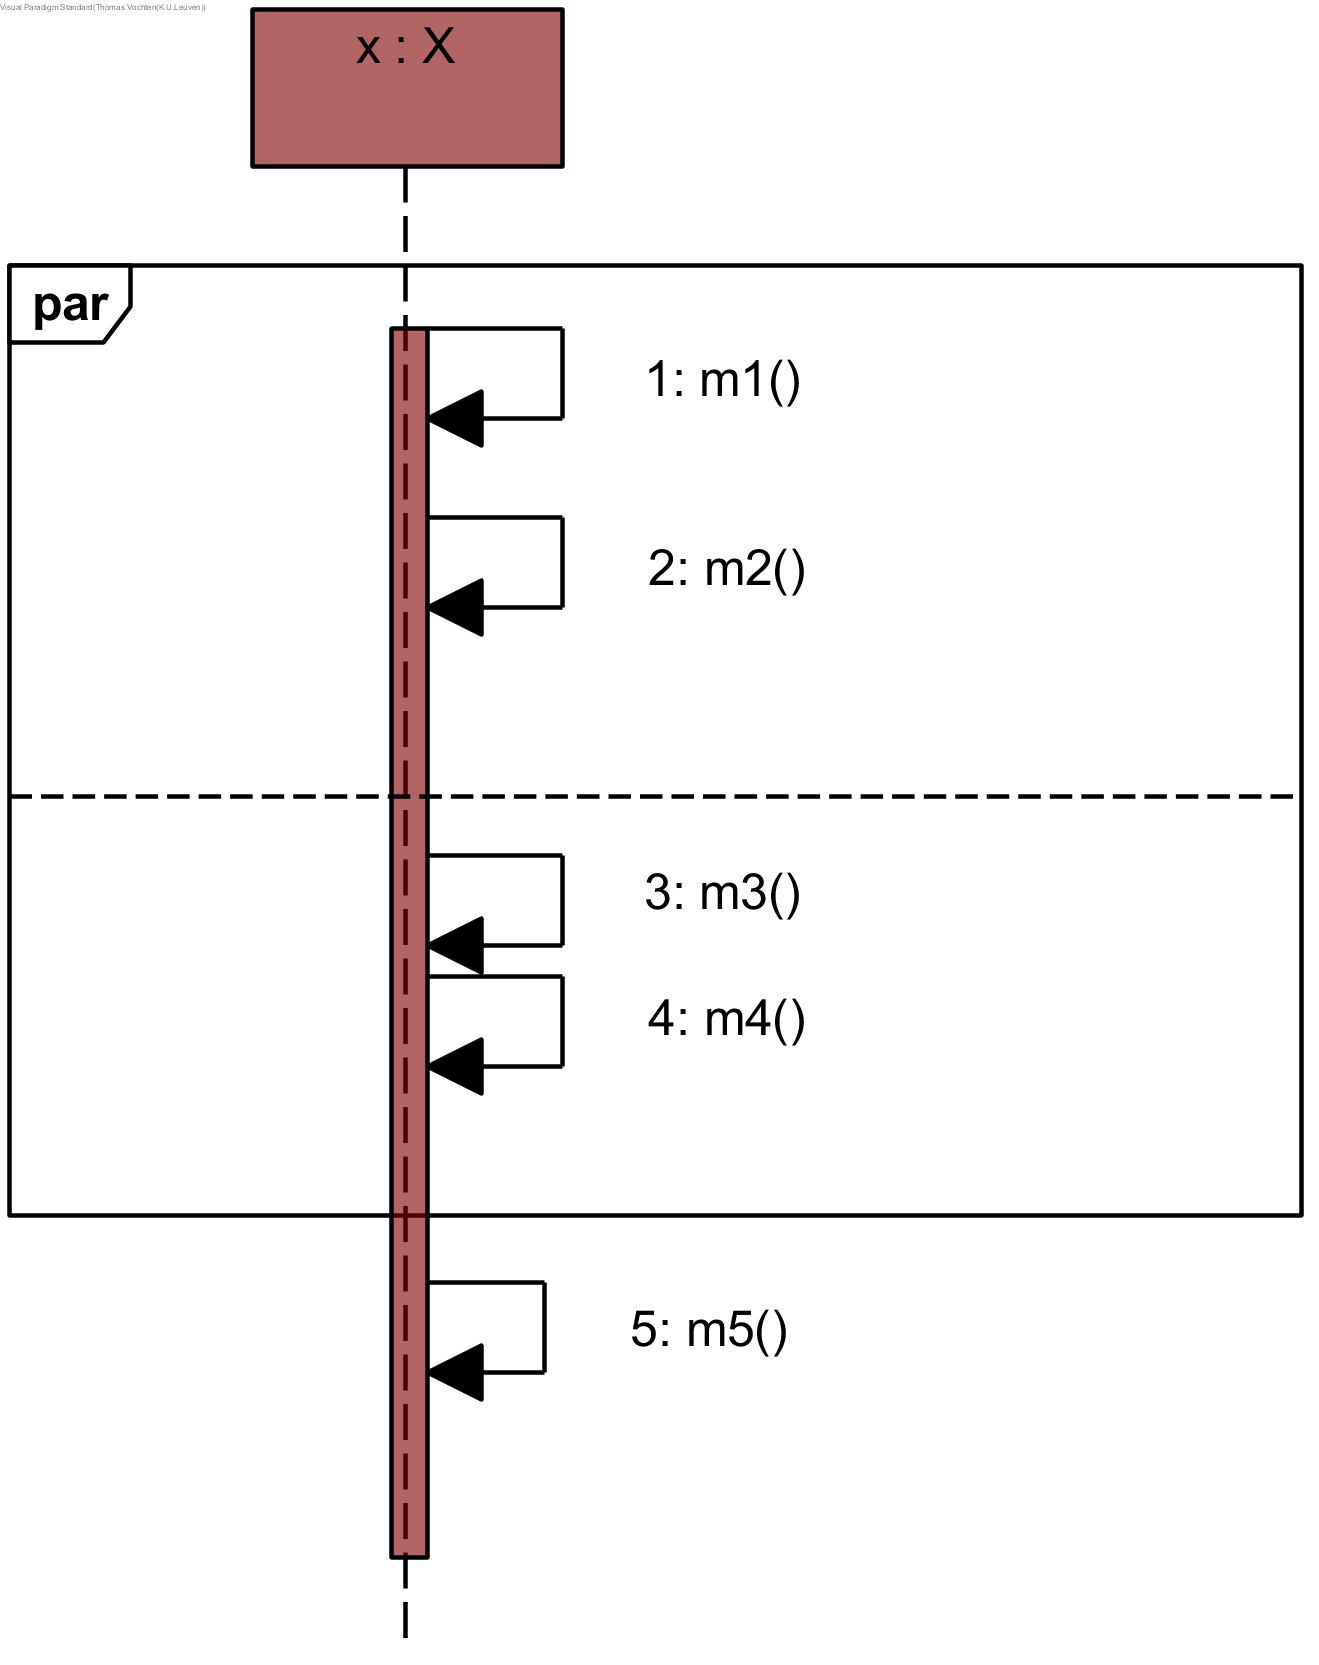
\includegraphics[width=0.6\textwidth]{chap-declaratieve-seq/seq-par.png}
	\caption{Een voorbeeld van het parallel gecombineerd fragment}
	\label{fig:seq-par}
\end{figure}

Zulk een fragment zou dus kunnen toelaten dat meer dan \'e\'en instructie tegelijk wordt uitgevoerd. Om zulke fragmenten te vertalen, zouden er toestandszinnen moeten komen voor \textit{SDPointAt/2} om bij binnenkomst in het fragment \textit{SDPointAt/2} waar te maken voor alle mogelijke eerste instructies van het fragment. Verder moet er een zin komen die stelt dat de uitvoering het fragment enkel kan verlaten als alle mogelijke laatste instructies zijn uitgevoerd.

\subsection{Een methode oproepen op meerdere objecten tegelijk}

Een andere denkpiste is het oproepen van een bepaalde methode op alle leden van een verzameling of de leden die aan een bepaald criterium voldoen. Zulke functionaliteit zou bijvoorbeeld toegepast kunnen worden om een sequentiediagram voor een booleaanse methode op te roepen op alle leden van een verzameling en om alle leden te selecteren waarvoor het resultaat \textit{true} is.

Er zijn meerdere mogelijke aanpakken om zulke functionaliteit te modelleren in LTC:

\begin{itemize}
	\item Laat toe dat alle methodes parallel kunnen worden uitgevoerd. Hiervoor is het echter noodzakelijk om objecten bij te houden als eigenaar van een bepaalde oproep aangezien de resultaten van een parallele oproep enkel betekenis hebben binnen de context waarin de parallele oproep gebeurt. Dit kan men doen door instanties een extra argument te maken van \textit{SDPointAt} en een nieuw predicaat te introduceren dat voor alle objecten betrokken in een parallele oproep bijhoudt welk object de eigenaar is van de oproep die de bron is van die parallele oproep. De predicaten voor diagramvariabelen, het predicaat \textit{ReturnPoint} en de functie \textit{CurrentStackLevel} moeten ook bijhouden voor welke oproep een bepaalde waarde geldt. Op die manier worden de resultaten van een parallele oproep steeds doorgegeven aan het juiste object. Men moet er echter voor zorgen dat de uitvoering niet springt naar de instructie direct na de parallelle oproep totdat de parallele oproep een resultaat heeft voor alle betrokken objecten. Deze aanpak zal waarschijnlijk een grote impact hebben op rekentijd en ruimtegebruik, maar het biedt de meest ruime mogelijkheden bij het ontwerpen van sequentiediagrammen.
	\item Markeer een methode expliciet als parallel uitvoerbaar en laat niet toe dat er een tijdens een parallele oproep een andere parallelle oproep gebeurt. Op deze manier vermijdt men de toevoeging van een extra argument aan \textit{SDPointAt/2} en extra predicaten die eigenaarschap van een oproep bijhouden. Men moet er enkel voor zorgen dat de resultaten van een parallele oproep hun juiste bestemming bereiken, bijvoorbeeld als er leden van een verzameling worden geselecteerd op basis van het resultaat van een booleaanse oproep of het toekennen van resultaten van een oproep van een methode die \textit{int} als resultaat heeft op alle leden van een verzameling aan een nieuwe verzameling. Deze aanpak zal waarschijnlijk een minder grote impact hebben op rekentijd en ruimtegebruik, maar dit beperkt de mogelijkheden bij het ontwerpen van sequentiediagrammen.
\end{itemize}

\section{Conclusie}

We vergeleken een rechtstreekse implementatie van Nim in LTC met de theorie gegenereerd uit het ontwerp in sectie \ref{sec:nim-design}. We merkten dat de LTC-theorie significant compacter was. Dit komt onder meer omdat sequentiediagrammen toelaten dat de toestand van maar \'e\'en variabele tegelijk wordt gecontroleerd. Verder heeft LTC enkel lussen in de vorm van iteratieve processen binnen het probleemdomein, waar sequentiediagrammen ook lussen moeten bevatten voor procedurale berekeningen. Deze observaties dienden als basis voor het ontwerpen van nieuwe soorten instructies voor sequentiediagrammen. De instructies integreren logica in de ontwerptaal voor sequentiediagrammen.

We maakten een nieuw ontwerp voor Nim waar we gebruikmaakten van deze instructies. Dit ontwerp vertaalden we naar een logische theorie. Modelexpansie en progressie\"inferentie waren significant performanter voor deze theorie vergeleken met de theorie uit sectie \ref{sec:nim-design}. Deze winst blijft grotendeels bewaard wanneer we ook toelaten dat de invulling van een associatie verandert over de tijd.

We gaven tenslotte een aanzet voor toekomstig onderzoek naar mogelijkheden om een methode op te roepen op meerdere objecten tegelijkertijd.